\documentclass{article}
\usepackage{listings}
\usepackage{mathrsfs}
\usepackage[utf8]{inputenc}
\usepackage{amssymb}
\usepackage{lipsum}
\usepackage{amsmath}
\usepackage{fancyhdr}
\usepackage{geometry}
\usepackage{scrextend}
\usepackage[english,german]{babel}
\usepackage{titling}
\setlength{\droptitle}{-3cm}
\usepackage{tikz}
\usepackage{algorithm,algpseudocode}
\usepackage[doublespacing]{setspace}
\usetikzlibrary{datavisualization}
\usetikzlibrary{datavisualization.formats.functions}
\usepackage{polynom}
\usepackage{amsmath}
\usepackage{gauss}
\usepackage{tkz-euclide}
\usetikzlibrary{datavisualization}
\usetikzlibrary{datavisualization.formats.functions}
\author{
Alexander Mattick Kennung: qi69dube\\
Kapitel 1
}
\usepackage{import}
\date{\today}
\geometry{a4paper, margin=2cm}
\usepackage{stackengine}
\parskip 1em
\newcommand\stackequal[2]{%
  \mathrel{\stackunder[2pt]{\stackon[4pt]{=}{$\scriptscriptstyle#1$}}{%
  $\scriptscriptstyle#2$}}
 }
\makeatletter
\renewcommand*\env@matrix[1][*\c@MaxMatrixCols c]{%
  \hskip -\arraycolsep
  \let\@ifnextchar\new@ifnextchar
  \array{#1}}
\makeatother
\lstset{
  language=haskell,
}
\lstnewenvironment{code}{\lstset{language=Haskell,basicstyle=\small}}{}
\usepackage{enumitem}
\setlist{nosep}
\usepackage{titlesec}

\titlespacing*{\subsection}{0pt}{2pt}{3pt}
\titlespacing*{\section}{0pt}{0pt}{5pt}
\titlespacing*{\subsubsection}{0pt}{1pt}{2pt}
\title{Vorlesung 4}


\begin{document}
	\maketitle
	LGS $Ax=b$ mit  $Dim(x)>Dim(m)$\\
	i.A. nicht lösbar!\\
	Aber man kann den $||Ax-b|| =mse(Ax,b)$ minimieren.\\
	$||Ax-b|| = \sqrt{<Ax-b,Ax-b>}$\\
	$\iff \frac{1}{2} <Ax-b,Ax-b>\to \min$\\
	$\iff \frac{1}{2} (<Ax,Ax-b>-<b,Ax-b>)\to \min$\\
	$\iff \frac{1}{2} (<Ax,Ax>-<Ax,b>-<b,Ax>+<b,b>)\to \min$\\
	$\stackrel{reelle Zahlen}{\iff} \frac{1}{2} (<Ax,Ax>-2<Ax,b>+<b,b>)\to \min$\\
	$\stackrel{reelle Zahlen}{\iff} \frac{1}{2} ((Ax)^TAx-2(Ax)^Tb+b^Tb)\to \min$\\
	$\stackrel{reelle Zahlen}{\iff} \frac{1}{2} (x^TA^TAx-2x^TA^Tb+b^Tb)\to \min$\\
	ableiten:\\
	$$\nabla (\frac{1}{2} (x^TA^TAx-2x^TA^Tb+b^Tb)) ) = \frac{1}{2}(2A^TAx-2A^Tb) = A^TAx-A^Tb\stackrel{!}{=}0\iff A^TAx = A^Tb$$
	Weil $A^TA$ positive definit ist (solange A vollen rang hat), ist $x$ das minimum (und nicht etwa max/plateu)\\
	1a)\\
	Punkte $(1,1), (3,2), (5,6), (7,8)$\\
	Gesucht gerade, die möglichst genau approximiert $g(x) = a_0+a_1x$\\
	$\begin{bmatrix}
		g(1)=&a_1+a_2*1 &= 1\\
		g(3)=&a_1+a_2*3 &= 2\\
		g(5)=&a_1+a_2*5 &= 6\\
		g(7)=&a_1+a_2*7 &= 8\\
	\end{bmatrix}$\\
	A= $\begin{bmatrix}
		1&1\\
		1&3\\
		1&5\\
		1&7\\
	\end{bmatrix}$\\
	$b =(1,2,6,8)^T$\\
	$x = (a_1,a_2)^T$\\
	Finde den best-fit mit Normalengleichung.\\
	$A^TA = \begin{bmatrix}
		4 &16\\
		16 &84
	\end{bmatrix}$
	$A^Tb =\begin{bmatrix}
		1&1\\
		1&3\\
		1&5\\
		1&7\\
	\end{bmatrix}^T (1,2,6,8)^T = (17,93)^T$\\
	Löse $A^TAx = A^Tb$\\
	$A^TA|b=\begin{bmatrix}
		4 &16&17\\
		16 &84&93
	\end{bmatrix}=\begin{bmatrix}
		4 &16&17\\
		0 &20&25
	\end{bmatrix}\implies a_2 = \frac{4}{5}, a_1 = -\frac{3}{4}$\\
	CCS-Format:\\
	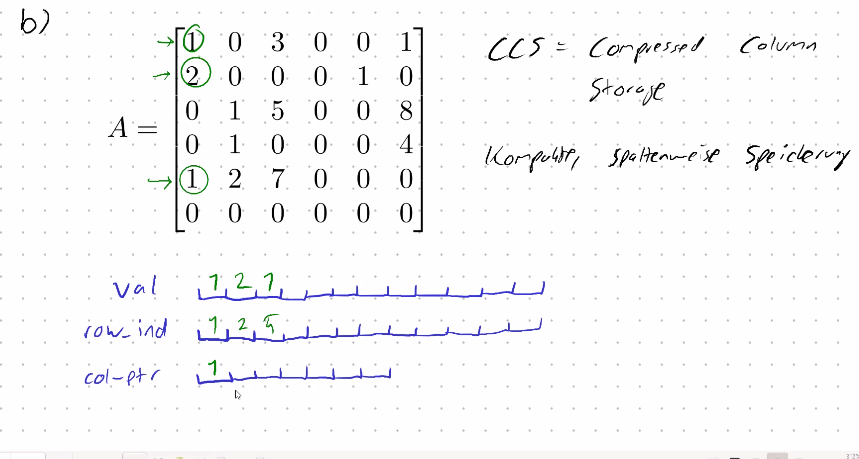
\includegraphics{CCS.png}
\end{document}